%%%%%%%%%%%%%%%
%
% $Autor: Wings $
% $Datum: 2020-01-29 07:55:27Z $
% $Pfad: General/SensorAPDS9960.tex
% $Version: 1785 $
%
%
%%%%%%%%%%%%%%%

\chapter{Sensormodul APDS-9960 for Gesture, Proximity, and Color Detection}

The APDS-9960 sensor, integrated on the Arduino Nano 33 BLE Sense, is a multifunctional optical sensor used for gesture recognition, ambient light detection, color sensing, and proximity measurement. The sensor uses an I²C interface for communication and comes equipped with an additional infrared LED.
\cite{Avago:2015}


\begin{center}    
	\begin{tikzpicture}
		\node at (0,0) (Board) {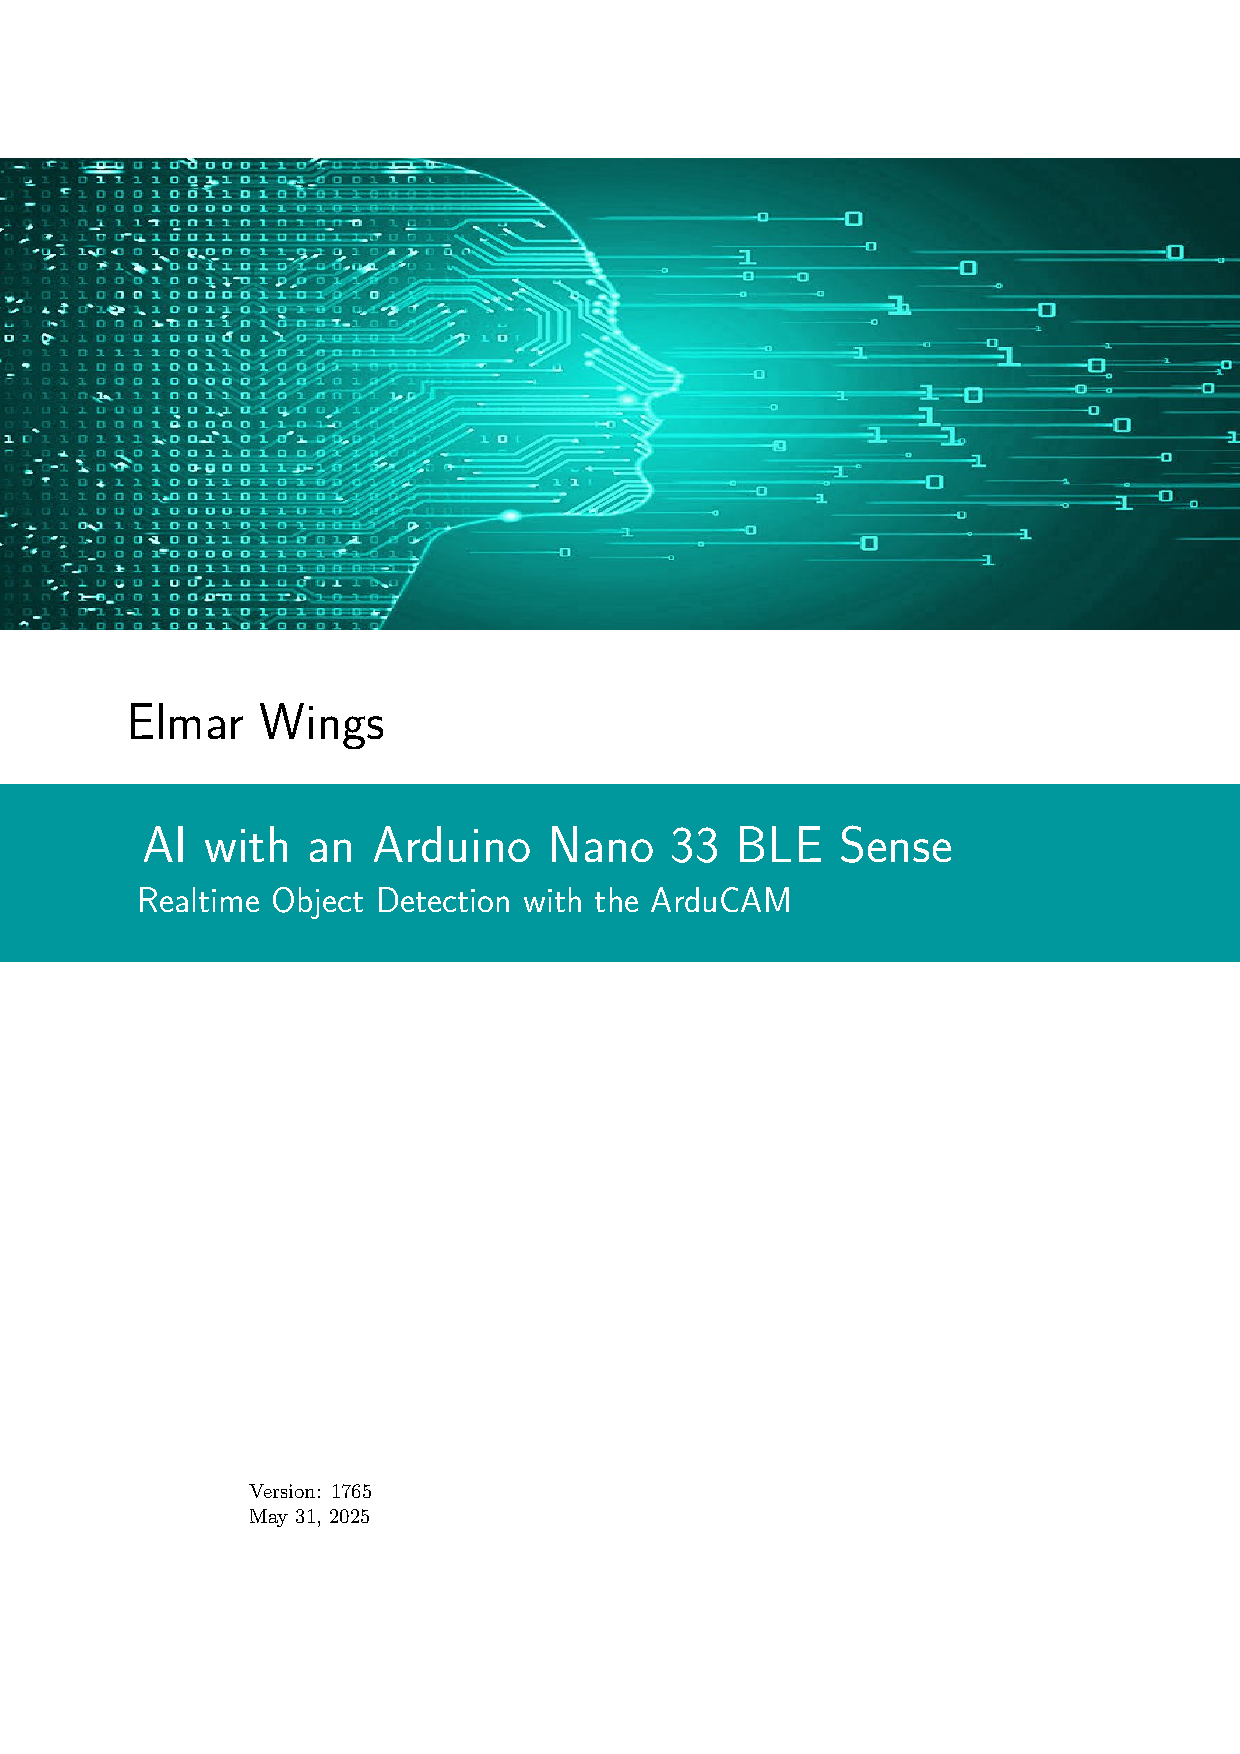
\includegraphics{Arduino/Nano33BLE/Nano33BLESense}};
		
		\fill[gray, opacity=0.7] (-6,-2.4) rectangle (6,2.4);
		
		\coordinate (A) at (-1,0.4);
		\coordinate (B) at (0.2,-0.2);    
		\begin{scope}
			\clip (A) rectangle (B);
			\node at (0,0) (Board) {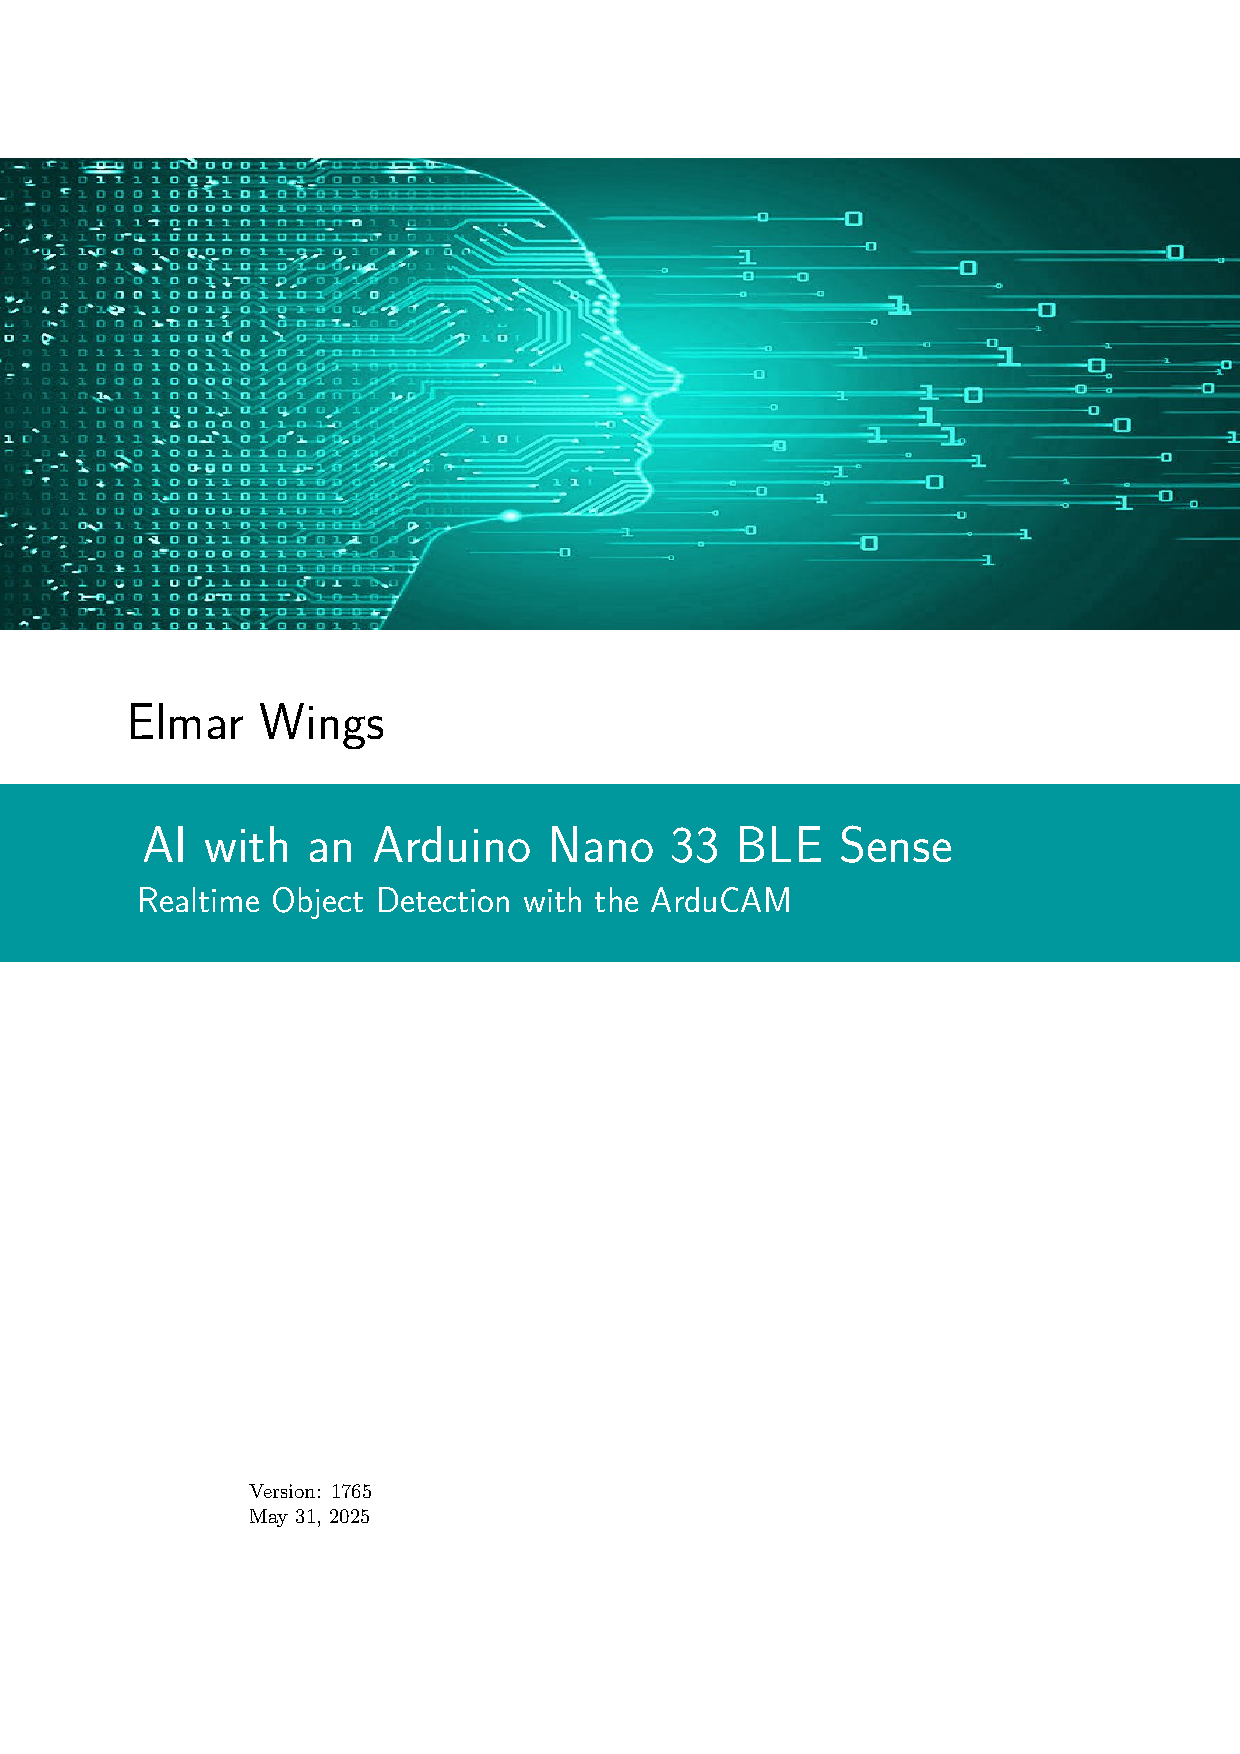
\includegraphics{Arduino/Nano33BLE/Nano33BLESense}};
		\end{scope}
		\draw[yellow,line width=2pt] (A) rectangle (B);
	\end{tikzpicture}    
	
	\captionof{figure}{Arduino Nano 33 BLE Sense's APDS-9960}
	\label{fig:5.1}
\end{center}

\bigskip


\Mynote{Figure 6.1 must be converted into a TikZ image to maintain consistency}

The sensor is located centrally on the Arduino Nano 33 BLE Sense, as indicated in the Figure \ref{fig:5.1}.










\section{Functionality of the APDS-9960}


The APDS-9960 is a versatile optical sensor that offers multiple functionalities, including color detection, proximity sensing, ambient light measurement, and gesture recognition. Each of these features plays a crucial role in various applications, ranging from smart lighting adjustments to touchless control systems.

In the following sections, each function of the APDS-9960 will be explored in detail, explaining its working principle, the type of data it provides, and its potential use cases.





\section{Key Technical Specifications}
\label{chap:Specification}

\subsection*{Power Supply}
\begin{itemize}
	\item Supply Voltage: 2.4 V to 3.6 V
	\item Maximum Voltage: 3.8 V
\end{itemize}

\subsection*{Power Consumption}
\begin{itemize}
	\item Active ALS Mode (Ambient Light Sensor): 200-250 µA
	\item Proximity and Gesture Modes: 790 µA (without LED)
	\item Sleep Mode: 1-10 µA
\end{itemize}

\subsection*{Temperature}
\begin{itemize}
	\item Operating Temperature Range: -30°C to +85°C
	\item Storage Temperature Range: -40°C to +85°C
\end{itemize}

\subsection*{Optical Properties}
\begin{itemize}
	\item LED Wavelength (max.): 950 nm
	\item LED Drive Current:
	\begin{itemize}
		\item 100 mA (Standard), 50 mA, 25 mA, 12.5 mA
		\item LED Boost Option: 100\%, 150\%, 200\%, 300\% (adjustable current boost)
	\end{itemize}
	\item Max Detection Distance for Color, Proximity and Gesture Sensor 0mm to 100mm
\end{itemize}

\subsection*{Proximity Sensor}
\begin{itemize}
	\item Pulse Width for Proximity Measurement: 4 µs to 32 µs
\end{itemize}

\subsection*{Gesture Sensor}
\begin{itemize}
	\item LED Pulse Count: 1 to 64 pulses
\end{itemize}

\subsection*{Connections}
\begin{itemize}
	\item I²C Communication:
	\begin{itemize}
		\item Data Rates: Up to 400 kHz
		\item Pins:
		\begin{itemize}
			\item SDA (I²C Data)
			\item SCL (I2C Clock)
			\item INT (Interrupt, Open Drain, Active Low)
			\item LDR (LED Driver Input)
		\end{itemize}
	\end{itemize}
\end{itemize}

\subsection*{Dimensions}
\begin{itemize}
	\item Length: 3.94mm
	\item Width: 2.36mm
	\item Height: 1.35mm
\end{itemize}

\cite{Avago:2015}


\section{Library \PYTHON{Arduino\_APDS9960}}

In the case of the APDS-9960 sensor, Arduino provides a library \FILE{Arduino\_APDS9960} for calling functions related to color detection, distance measurement, or gesture recognition.

The library for the sensor is \FILE{Arduino\_APDS9960}. This allows measuring gestures, colors, light intensity, and distances with the sensor. Communication between the Arduino Nano 33 BLE Sense's chip and the APDS-9960 module occurs via an internal I²C interface \cite{Avago:2015}.

The library is included by using the command \PYTHON{\#include <Arduino\_APDS9960.h>}.






\subsection{Installation of APDS-9960 Library}

The library is installed as follows:



\begin{enumerate}
	\item Open the Arduino IDE and navigate to \menu[,]{Tools,Manage Libraries...}.
	\item In the Library Manager, use the search bar to look for "Arduino\_APDS9960".
	\item Several libraries will be displayed. Select the library titled "Arduino\_APDS9960" by Arduino and click \textit{Install}.
	\item Once installed, the IDE will show a message in the console confirming the installation. The "Install" button will also change to "Remove", as seen in Figure \ref{fig:APDS9960}, indicating the library is ready for use.
\end{enumerate}


\begin{center}
	\includegraphics[width=8cm]{Arduino/APDS9960/APDS9960Installed.png}
	\captionof{figure}{APDS-9960 Library Instalation}\label{fig:APDS9960}		
\end{center} 










\subsection{Functions}

After the theoretical overview of the APDS-9960 sensor's functions, the following section will explain the practical implementations. It will demonstrate how the various functions of the sensor, such as color detection, gesture recognition, and proximity sensing, can be applied in practice to activate and evaluate the sensor's capabilities.

\medskip

Here are the codes to utilize the various functions of the APDS-9960 sensor, such as color detection, gesture recognition, and proximity sensing, see \cite{ArduinoAPDS9960:2024}:

\begin{itemize}
	\item \PYTHON{begin()}: The \PYTHON{begin()} method activates and initializes the APDS9960 sensor. It is typically called during the \PYTHON{setup\{\}} phase.
	
	\medskip
	
	\begin{itemize}
		\item Return value \PYTHON{TRUE}: Initialization was successful.
		\item Return value \PYTHON{FALSE}: Initialization failed.
	\end{itemize}
	
	\item \PYTHON{end()}: The \PYTHON{end()} method deactivates the APDS9960 sensor.
	
	
	\item \PYTHON{colorAvailable()}: This method checks if color data is available to be retrieved.
	
	\medskip
	
	\begin{itemize}
		\item Return value \PYTHON{TRUE}: Color data is available.
		\item Return value \PYTHON{FALSE}: No color data is available.
	\end{itemize}
	
	\item \PYTHON{readColor(...)}: This method retrieves the color values from the sensor.
	
	It can either read just the color values or the color values along with the ambient light intensity.
	
	\medskip
	
	To read only the color values:
	
	\PYTHON{int r, g, b;}
	
	\PYTHON{APDS.readColor(r, g, b);}
	
	\medskip
	
	The variables \PYTHON{r}, \PYTHON{g}, and \PYTHON{b} will contain the updated color values. The value range is $0, 1, 2, \ldots, 255$.
	
	\medskip
	
	To read both the color values and ambient light intensity:
	
	\PYTHON{int r, g, b, a;} 
	
	\PYTHON{APDS.readColor(r, g, b, a);}
	
	\medskip
	
	The variables \PYTHON{r}, \PYTHON{g}, and \PYTHON{b} will contain the updated color values, while \PYTHON{a} will contain the ambient light intensity. The value range is $0, 1, 2, \ldots, 255$.
	
	\item \PYTHON{proximityAvailable()}: This method checks if proximity data is available.
	
	\medskip
	
	\begin{itemize}
		\item Return value \PYTHON{TRUE}: Proximity data is available.
		\item Return value \PYTHON{FALSE}: No proximity data is available.
	\end{itemize}
	
	\item \PYTHON{readProximity()}: This method reads the proximity value.
	
	\medskip
	
	\begin{itemize}
		\item Return value \PYTHON{int proximity = APDS.readProximity()}: Returns the proximity value.
		\item Return value \PYTHON{-1}: Proximity could not be determined.
	\end{itemize}
	
	\item \PYTHON{gestureAvailable()}: This method checks if a gesture has been detected.
	
	\medskip
	
	\begin{itemize}
		\item Return value \PYTHON{TRUE}: A gesture has been detected.
		\item Return value \PYTHON{FALSE}: No gesture detected.
	\end{itemize}
	
	\item \PYTHON{setGestureSensitivity()}: Gesture detection is influenced by lighting conditions, speed, and distance of movement. This function allows you to adjust the sensitivity of gesture recognition. A higher value detects more gestures, but increases the chance of false positives. A lower value reduces the likelihood of detecting gestures.
	
	The valid range is \PYTHON{1} to \PYTHON{100}.
	
	The default value is \PYTHON{80}.
	
	\item \PYTHON{readGesture()}: If a gesture has been detected, it can be retrieved using the \PYTHON{readGesture()} method. The possible return values are:
	
	\begin{itemize}
		\item \PYTHON{GESTURE\_UP}: An upward movement has been detected.
		\item \PYTHON{GESTURE\_DOWN}: A downward movement has been detected.
		\item \PYTHON{GESTURE\_LEFT}: A leftward movement has been detected.
		\item \PYTHON{GESTURE\_RIGHT}: A rightward movement has been detected.
		\item \PYTHON{GESTURE\_NONE}: No gesture has been detected.
	\end{itemize}
	
	\item \PYTHON{setInterruptPin()}: This method sets the pin used to trigger a measurement. The pin is usually detected automatically, but can be set manually using this function.
	
	If \PYTHON{-1} is passed, no pin is connected.
	
	If \PYTHON{0} or a higher value is passed, that pin will be used.
	
	The default value depends on the board.
	
	\item \PYTHON{setLEDBoost(...)}: The sensor includes an infrared LED that can be temporarily boosted to provide higher brightness. It can be set to provide up to 300\% of its normal power. This can be configured using this method.
	
	\medskip
	
	Usage:
	
	\begin{itemize}
		\item \PYTHON{0}: Boost to 100\% (default power).
		\item \PYTHON{1}: Boost to 150\%.
		\item \PYTHON{2}: Boost to 200\%.
		\item \PYTHON{3}: Boost to 300\%.
	\end{itemize}    
	
	\medskip
	
	Return values:
	
	\begin{itemize}
		\item \PYTHON{0}: Failure.
		\item \PYTHON{1}: Success.
	\end{itemize}
\end{itemize}




\section{Simple Function Tests}

The following code examples can be used to test and try out all functions of the APDS-9960.

\subsection{Example Color Detection}

The library  \PYTHON{Arduino\_APDS9960} includes an example code demonstrating how to perform color detection with the sensor APDS-9960 on an Arduino Nano 33 BLE Sense. This example also tests the ambient light sensor, as both functionalities rely on the same underlying technology. The measured color channel intensities (Red, Green, and Blue) are displayed in the Serial Monitor for real-time observation.

The sensor APDS-9960 enables accurate RGB color detection by measuring the intensity of red, green, and blue light reflected from an object. These values can be visualized in the Serial Plotter, allowing users to track changes in color intensity over time through a graphical representation. This feature is particularly useful for applications that require real-time color monitoring or dynamic light adjustments.


\subsection{Example Color Detection - Manual}

\Mynote{to do}


\subsection{Setting Up the Color Sensor Measurement Program}

To begin the process of creating the color sensor measurement program, open the Arduino Cloud Editor and navigate to the "Libraries" tab. Search for the "Arduino-APDS9960" library and download it. Afterward, click on "More info" to access the GitHub repository, where several examples are provided.

Next, connect the Arduino Nano 33 BLE Sense to the computer, ensuring that the Cloud Editor detects both the board and the corresponding port. If the board is not automatically recognized, follow the instructions to install the necessary plugin to enable the editor to detect the board. Confirm that the correct port is selected. Finally, upload the program to the Arduino, and by opening the serial monitor, the measured values will be recorded in the Arduino IDE.

\subsection{Example }Color Detection - Code}

First, serial communication is started with \PYTHON{Serial.begin(9600)} to send data to the computer. The command  \PYTHON{APDS.begin()} initializes the sensor and in the event of a potential error, an error message is output via the serial interface.

\bigskip



\bigskip

The code operates within the function \PYTHON{loop()} of a sketch to continuously read and display color values from the APDS-9960 sensor. Initially, it checks if a color reading is available by using the method \PYTHON{APDS.colorAvailable()}. If no reading is available, the program briefly pauses for 5 milliseconds to avoid excessive CPU usage. Once a reading is ready, the method \PYTHON{APDS.readColor(r, g, b)} retrieves the color data and stores the red, green, and blue values in the respective variables. These values are then printed to the Serial Monitor, labeled clearly as ``r'', ``g'', and ``b''. A one-second delay is added before the program repeats the loop, allowing for clear intervals between consecutive readings.




\subsection{Example Color Detection - File}

The program can be found at 

\medskip

{
	\captionof{code}{Simple sketch using the sensor APDS9960 for colors}\label{TestAPDS9960Color}
	\ArduinoExternal{}{../../Code/Nano33BLESense/APDS9960/TestAPDS9960Color/TestAPDS9960Color.ino}
}


\subsection{Proximity}

A simple code for testing the proximity sensor is also provided by the library. The proximity sensor is designed for measuring distances of up to 100mm.

\subsection{Proximity - Manual}

Open the Arduino Cloud Editor and navigate to the Libraries tab. In the search bar, search for the library \PYTHON{Arduino\_APDS9960}. Once located, open the Examples section within the library and select the sketch ``ProximitySensor''.
\smallskip
Connect the Arduino Nano 33 BLE Sense to the computer. Check that the Cloud Editor recognizes the board by verifying if both the board and port are listed in the dropdown menu.

\subsection{Example Proximity - Code}

First, serial communication is started with \PYTHON{Serial.begin(9600)} to send data to the computer. The method \PYTHON{APDS.begin()}  initializes the sensor and in the event of a potential error, an error message is output via the serial interface.


\bigskip


The code operates within the function \PYTHON{loop()}  of a sketch to continuously read and display proximity values from the sensor APDS-9960. It begins by checking if a proximity reading is available using the method \PYTHON{APDS.proximityAvailable()}. If a reading is ready, the method \PYTHON{APDS.readProximity()} retrieves the proximity value, where \PYTHON{0} indicates a close object, \PYTHON{255} indicates a distant object, and \PYTHON{-1} signals an error in reading. This proximity value is then printed to the Serial Monitor. A delay of 100 milliseconds is added before the program repeats the loop, ensuring a brief interval between consecutive readings.


\subsection{Example Proximity - File}

The sketch can be found at 

\bigskip

{
	\captionof{code}{Simple sketch using the sensor APDS9960 for measuring the proximity}\label{TestAPDS9960Proximity}
	\ArduinoExternal{}{../../Code/Nano33BLESense/APDS9960/TestAPDS9960Proximity/TestAPDS9960Proximity.ino}
}

\subsection{Gesture Detection}
\subsection{Example Gesture Detection}

The library \FILE{Arduino\_APDS9960} also provides an example sketch demonstrating gesture detection with the sensor APDS-9960 on an Arduino Nano 33 BLE Sense. Some LED feedback signals have been programmed to provide quick visual feedback.

\subsection{Example Gesture Detection - Manual}

\Mynote{to do}


\subsection{Example Gesture Detection - Code}

In this example sketch, the library \FILE{Arduino\_APDS9960} is integrated first and then the setup is created. In addition, the LED pins are configured so that they behave as outputs.


\bigskip

After that, serial communication is initialized, and the program verifies whether the sensor is correctly initialized using \PYTHON{APDS.begin()}. If initialization fails, an error message is printed. The gesture sensitivity can be adjusted via \PYTHON{APDS.setGestureSensitivity(value)}, where values range from 1 to 100, affecting detection accuracy and sensitivity. The sketch sets a default sensitivity and signals the start of gesture detection by turning off the RGB LEDs with \PYTHON{digitalWrite(LEDR, HIGH)}, \PYTHON{digitalWrite(LEDG, HIGH)}, and \PYTHON{digitalWrite(LEDB, HIGH)}.

In the function \PYTHON{loop()}, the code continuously checks for available gestures using \PYTHON{APDS.gestureAvailable()}. When a gesture is detected, it is read using \PYTHON{APDS.readGesture()} and interpreted within a \PYTHON{switch} statement. Each gesture corresponds to specific LED behavior:

\begin{itemize}
	\item \PYTHON{GESTURE\_UP}: The red LED is briefly turned on, then off after a 1-second delay.
	\item \PYTHON{GESTURE\_DOWN}: The green LED is briefly turned on, then off after a 1-second delay.
	\item \PYTHON{GESTURE\_LEFT}: The blue LED is briefly turned on, then off after a 1-second delay.
	\item \PYTHON{GESTURE\_RIGHT}: All LEDs are turned on simultaneously, then off after a 1-second delay.
\end{itemize}

The \PYTHON{default} case ensures no action if an undefined gesture is detected.



\subsection{Example Gesture Detection - File}

The sketch can be found at 

\bigskip

{
	\captionof{code}{Simple sketch using the sensor APDS9960 for gesture detection}\label{TestAPDS9960Gesture}
	\ArduinoExternal{}{../../Code/Nano33BLESense/APDS9960/TestAPDS9960Gesture/TestAPDS9960Gesture.ino}
}

\subsection{Troubleshoot}


Errors in color detection can be caused by insufficient lighting in the room. Please ensure that the environment is bright enough for the color detection function.


\section{Calibration Color Detection}

\section{Calibration Color Detection}

Due to variations in environmental light conditions and the sensitivity of the sensor, calibration is required to ensure accurate color detection. This section outlines the calibration process using a standard color chart under constant lighting conditions. To carry out the calibration, the Arduino, a connection cable (USB A to USB Micro), and a laptop or computer with the appropriate Arduino development environment are required.

\medskip

The proximity and gesture feature is pre-configured and factory-calibrated to detect proximity and gesture at a distance of 100mm, eliminating the need for customer calibration.
\cite{BroadcomAPDS9960:2024}

\subsection{Calibration Setup}

A standardized color chart is used, which provides reference values for perfect red, green, and blue under constant lighting conditions. The RGB values from the sensor are read as raw, uncalibrated data, which must be normalized to a standard range (0–255) for accurate color detection.\Mynote{citation, picture}

\subsection{Step 1: Measuring Reference Values}

The first step in the calibration process is to measure the raw sensor values for each primary color (red, green, and blue) using the standardized color chart. By placing the color chart in front of the sensor and reading the raw RGB values, we can establish the maximum possible sensor readings for each color channel.

\[
\text{RawRed} = \max(R_{\text{measured}})
\]
\[
\text{RawGreen} = \max(G_{\text{measured}})
\]
\[
\text{RawBlue} = \max(B_{\text{measured}})
\]

These maximum values are obtained by positioning the chart at a fixed distance of one centimeter and ensuring constant light intensity.

\subsection{Step 2: Normalizing the Sensor Values}
Once the maximum sensor readings for red, green, and blue are obtained, the raw sensor data is normalized to a 0-255 scale. This ensures that the sensor's readings correspond to standard RGB values. The following formula is used for normalization:

\[
R_{\text{calibrated}} = \frac{R_{\text{raw}}}{\text{RawRed}} \times 255
\]
\[
G_{\text{calibrated}} = \frac{G_{\text{raw}}}{\text{RawGreen}} \times 255
\]
\[
B_{\text{calibrated}} = \frac{B_{\text{raw}}}{\text{RawBlue}} \times 255
\]

Where:

\begin{itemize}
	\item $R_{\text{raw}}, G_{\text{raw}}, B_{\text{raw}}$ are the raw sensor values for each channel.
	\item $\text{RawRed}, \text{RawGreen}, \text{RawBlue}$ are the maximum measured values from the standard color chart.
\end{itemize}

\subsection{Step 3: Implementing the Calibration in Code}

The normalization process is implemented directly in the Arduino code to adjust the sensor's readings. To begin calibration, open the Serial Monitor, enter ``OK'' in the command line, and press Enter to confirm. The following steps will then be explained through text output.

\bigskip

After the user initiates the calibration by typing ``OK'' into the Serial Monitor, the sketch starts. The sketch guides the user through the calibration of red, green, and blue colors, with each phase confirmed by entering ``OK''. The pins for the RGB LEDs are defined, and variables store the maximum calibration values for each color. Status variables control the sequence, ensuring each phase is completed before moving to the next. These maximum values are later used for accurate color detection in the Application code.

\bigskip


The following code section begins by initializing serial communication at a baud rate of 9600, enabling interaction through the serial monitor. Next, it sets the RGB LED pins as outputs and turns on all LEDs to create white light, which helps capture accurate color measurements. The code then initializes the sensor APDS-9960, checking for successful setup. If the sensor fails to initialize, an error message is printed, and the program halts. If successful, a message confirms initialization and prompts the user to type ``OK'' in the serial monitor to proceed with the calibration process explanation.

\bigskip

The next code segment in the loop first checks if the user has entered ``OK'' to start the calibration process. After confirmation, it displays an explanation and instructions. After showing the explanation, it waits for the user to confirm by typing ``OK'' again, which then initiates the red color calibration by prompting the user to place the red chart in front of the sensor. The loop pauses at each step until the user confirms.

\Mynote{Screen shot?}

\bigskip

Each color calibration starts after the user types ``OK'' in the Serial Monitor. The sketch measures the highest detected value for each color over 10 seconds and sets it as the calibration maximum. After all colors are calibrated, it displays the final maximum values for red, green, and blue in the Serial Monitor, completing the process. The \PYTHON{maxRed}, \PYTHON{maxGreen}, and \PYTHON{maxBlue} values can later be entered into the application sketch to apply the calibration to the sketch.


\subsection{Calibration File}

The sketch can be found at 

\bigskip

{
	\captionof{code}{APDS-9960: Example Calibration}
	\ArduinoExternal{}{../../Code/Nano33BLESense/APDS9960/APDS9960Calibration/APDS9960Calibration.ino}
}


\subsection{Step 4: Validating the Calibration}

To ensure the calibration is successful, the sensor readings should be tested again using the standard color chart. The calibrated values for red, green, and blue should be close to 255 for the respective pure colors on the chart. If the readings deviate significantly, further adjustment of the maximum reference values may be necessary.

\bigskip

The calibration of the sensor APDS-9960 is essential for accurate RGB detection. By using a standard color chart and constant lighting conditions, the sensor's raw values can be normalized to provide consistent and reliable color readings. This process can be further refined by adjusting for specific environmental factors or sensor placement.


\section{Tests}

\subsection{Simple Function Test}

\subsection{Test all Functions}

\section{Simple Application}

Similarly, by following all the steps for uploading and compiling the sketch we can see the results of sensor APDS-9960  on Serial Monitor, too. For seeing the different output, we can change the input for the sensor too, e.g: for color detection we can switch the colors, for gesture detection we can also switch the gestures, and for proximity also do the same. The resulted output as shown in the figure.  \ref{fig:2} 

\Mynote{rewrite and extend}

\begin{center}
	\includegraphics[width=9.5cm]{Nano33BLESense/APDS-Output}
	\captionof{figure}{Gesture, Proximity, Color Sensor Output Window}
	\label{fig:2}
\end{center}

We can also run the single funcnality of this sensor too, e.g; if we just need to capture the color of product, we can also run the color detection program. It depends upon the application and we can implement our application and modify the code as per our desire results.


{
	\captionof{code}{Simple sketch using the sensor APDS9960}\label{TestAPDS9960}
	\ArduinoExternal{}{../../Code/Nano33BLESense/APDS9960/TestAPDS9960/TestAPDS9960.ino}
}




%%%%%%%%%%%%%%%%%%%%%%%%%%%%%%%%%%


\section{Further Readings}

\begin{itemize}
	%    \item S. Grzesik, R. Kluwak, and B. Plikusinski, "Multispectral Sensor Application Possibility Research for Temperature Measurement," \textit{2023 23rd International Conference on Mechatronics - Mechatronika (ME)}, Brno, Czech Republic, pp. 1-6, 2023. Available at: \url{https://ieeexplore.ieee.org/document/10349583}
	
	\item SparkFun Electronics, ``APDS-9960 RGB and Gesture Sensor Hookup Guide''. A comprehensive guide that explains the functionality of the APDS-9960 and provides step-by-step instructions for implementation. Available at: \url{https://learn.sparkfun.com/tutorials/apds-9960-rgb-and-gesture-sensor-hookup-guide/all}, \cite{Hymel:2024}
	
	\item Maker Guides, ``APDS-9960 Gesture and Color Sensor with Arduino''. This tutorial provides a hands-on introduction to using the APDS-9960 sensor with Arduino, including gesture and color recognition. Available at: \url{https://www.makerguides.com/apds-9960-gesture-and-color-sensor-with-arduino/}, \cite{Maetschke:2024}
\end{itemize}



